\documentclass[11pt]{article}

\usepackage[margin=1in]{geometry}
\usepackage{amsmath,amssymb,booktabs,longtable,array}
\usepackage{enumitem}
\usepackage{float}
\usepackage[hidelinks]{hyperref}
\usepackage{listings}
\usepackage{microtype}
\usepackage{siunitx}
\usepackage{xcolor}
\usepackage{tikz}
\usetikzlibrary{arrows.meta,positioning,shapes.geometric}

\newcommand{\R}{\mathbb{R}}
\newcommand{\norm}[1]{\left\lVert #1\right\rVert_2}
\newcommand{\abs}[1]{\left\lvert #1\right\rvert}
\newcommand{\code}[1]{\texttt{#1}}
\newcommand{\measured}{\textsc{measured}}
\newcommand{\expected}{\textsc{expected}}
\newcolumntype{L}[1]{>{\raggedright\arraybackslash}p{#1}}

\lstdefinestyle{reportlisting}{
  basicstyle=\ttfamily\small,
  columns=fullflexible,
  frame=single,
  framerule=0.3pt,
  breaklines=true,
  keepspaces=true,
  showstringspaces=false,
  xleftmargin=1em,
  xrightmargin=1em
}
\lstset{style=reportlisting}

\title{Adaptive Acceleration of Thermochimica Equilibrium Calculations in MOOSE:\\
Algorithms, Scaling, Performance, and Benchmark Evaluation}
\author{MOOSE Chemical Reactions Module}
\date{Technical report, 28 July 2026}

\begin{document}
\maketitle

\begin{abstract}
Thermochimica computes multiphase thermodynamic equilibrium by Gibbs-energy minimization (GEM).
Repeated GEM evaluations can dominate a multiphysics calculation when the equilibrium map is
queried at every mesh entity and time step.  The MOOSE implementation evaluated here reduces GEM
calls through worker-local in-situ tabulation and one of two safeguarded mappings: phase-aware
inverse-distance interpolation or a fixed-assemblage Karush--Kuhn--Tucker (KKT) sensitivity
predictor with an adaptive ellipsoid of accuracy.  A prediction is published only after
model-specific regime, geometry, empirical-error, complementarity, and physical-invariant checks;
otherwise, execution falls back to exact GEM.  Periodic audits always publish the exact value.

The repository contains a comprehensive benchmark design but no successful production campaign.
The available 144-row HPC failure file records a pre-solve command-construction defect rather
than performance data.  After the repository's targeted repair, a one-repetition local study
showed KKT worker-time speedups of approximately \(7.3\)--\(7.5\) in smooth single-phase Mo--Ru
windows at 1,000 states, while total wall speedups remained \(1.4\)--\(1.6\) because fixed
application overhead dominated.  The same exploratory study showed conservative fallback in
two-phase and full-traversal problems, no audit or state-restoration failures, and normalized
sample errors below unity.  A separate scaling study exposed grid aliasing at 10,000 states:
9,926 query points became exact cache reuses.  Those points measure lookup performance, not
surrogate interpolation.  This report defines the algorithms, derives their computational and
memory scaling, evaluates the experimental design and implementation, reports the available
evidence without conflating it with production measurements, and specifies the results expected
from a statistically controlled HPC rerun.  Exact mode remains the default.
\end{abstract}

\tableofcontents

\section{Executive assessment}

The implementation is technically substantial and, in its fail-closed behavior, appropriately
conservative for a thermodynamic kernel embedded in multiphysics software.  The strongest aspects
are the isolation of stateful Fortran execution in worker processes, exact fallback on every
rejection path, explicit active-regime tokens for the KKT method, deterministic exact auditing,
transactional state restoration, exhaustive sampled-output comparison, and correctness-gated
performance profiles.  The test catalog covers exact reuse, interpolation, auditing, cache
saturation, KKT retrieval, phase-boundary behavior, unsupported-model fallback, and the historical
Li--F state-contamination reproducer.

The principal qualification gaps are experimental rather than conceptual:
\begin{enumerate}[leftmargin=*]
  \item the submitted full capability campaign produced 144 failures and no timings;
  \item the executable is recorded by path but not by digest or build provenance, so source and
  binary identity are not cryptographically tied;
  \item the large points in the fixed-HCP mesh study contain training/query grid overlap and
  therefore confound exact reuse with interpolation scaling;
  \item one upstream Thermochimica sensitivity test still references a removed MSTDB v3 example
  file and fails in the present checkout; and
  \item no full-tier, seven-repetition result set is present, so confidence intervals, HPC
  topology effects, and high-dimensional fluoride performance remain prospective.
\end{enumerate}

The scientifically defensible conclusion is therefore narrower than ``the method is faster.''
The source and local exploratory evidence support the algorithmic mechanisms, fail-closed safety,
and strong reductions in the GEM portion of smooth eligible workloads.  They do not yet establish
portable end-to-end speedup.  Publication claims should be conditioned on successful full-tier
runs, non-overlapping trajectories, archived executable provenance, and correctness gates applied
before timing comparisons.

\section{Problem statement}

Let $T$ and $P$ denote temperature and pressure, and let
$\boldsymbol{a}=(a_1,\ldots,a_n)^T$ contain nonnegative elemental inputs.  Abstractly,
Thermochimica solves a constrained equilibrium problem of the form
\begin{equation}
  \boldsymbol{n}^{\star}(T,P,\boldsymbol{a})
  \in \underset{\boldsymbol{n}\geq 0}{\operatorname{argmin}}
  \;G(T,P,\boldsymbol{n})
  \quad\text{subject to}\quad
  \mathbf{A}\boldsymbol{n}=\boldsymbol{a},
  \label{eq:gem}
\end{equation}
where $\boldsymbol{n}$ represents phase and species amounts and $\mathbf{A}$ enforces elemental
conservation.  The configured output map is
\begin{equation}
  \boldsymbol{y}=\mathcal{F}(T,P,\boldsymbol{a})\in\R^m.
  \label{eq:map}
\end{equation}
It may contain phase or species amounts, fractions, potentials, pressures, Gibbs energies, driving
forces, and integral system properties.

Within a fixed active phase assemblage, $\mathcal{F}$ is often locally smooth.  At a phase
boundary its derivatives may change abruptly and an output may appear or disappear.  The adaptive
method therefore treats a canonical phase assemblage as a discrete local regime rather than
assuming that one globally smooth surrogate exists.

The method is an in-situ tabulation algorithm: it learns only from exact states visited by the
simulation.  It does not train an offline model and it does not alter the thermodynamic database or
the GEM equations.

\section{Repository architecture and execution model}

\subsection{Software layers}

The capability spans three software layers, each with a distinct responsibility:
\begin{description}[style=nextline]
  \item[MOOSE action and configuration]
  \code{ChemicalCompositionAction.C} validates user parameters, constructs typed output
  descriptors, classifies outputs as extensive, nonnegative, or fractional, and transfers the
  immutable configuration to the executor.
  \item[MOOSE executor]
  \code{ThermochimicaData.C} batches mesh-entity inputs, owns cache and surrogate logic, launches
  isolated worker processes, evaluates requested outputs, performs auditing, and aggregates
  telemetry.
  \item[Thermochimica sensitivity API]
  \code{EquilibriumSensitivity.f90} captures and restores converged module state, forms the
  fixed-assemblage residual and its derivatives, equilibrates and factors the KKT matrix, and
  exposes diagnostics through C and C++ interfaces.
\end{description}
The Python driver \code{benchmark.py}, JSON manifests, MOOSE input files, Slurm launchers, plotting
style, and result-reporting logic form a fourth, experimental layer.  It does not participate in
production equilibrium evaluation.

\subsection{Process isolation and batching}

Thermochimica stores equilibrium data in Fortran modules and is not intrinsically reentrant.
Each threaded MOOSE object therefore forks an isolated worker process.  Parent and worker exchange
commands over a socket and exchange batched identifiers, inputs, results, row status, and
telemetry through shared memory.  For a batch of \(B\) states with input width \(d\) and output
width \(m\), parent-side packing and result movement are \(O(B(d+m))\); these costs are outside the
reported worker solve time but inside application wall time.

Each worker owns its cache, audit sequence, previous-solve state, and sensitivity records.  This
eliminates locks in the thermodynamic hot path and prevents Fortran state races.  It also means
that cache training, memory, and exact fallback are replicated across workers.  A change from one
thread or rank to \(p\) workers changes the state history seen by each cache and can therefore
change the exact-call count even for a fixed global mesh.

\subsection{Benchmark state trajectory}

The benchmark coordinate \(x\in[0,1]\) is a state generator, not a physical spatial coordinate.
With \code{nx} \(=N\), one Thermochimica execution stage evaluates \(N\) independent equilibria.
The input files use two transient steps to accommodate MOOSE execution ordering:
\begin{enumerate}[leftmargin=*]
  \item an initial trajectory populates the cache;
  \item auxiliary variables write a displaced trajectory; and
  \item the final stage evaluates that displaced trajectory as the post-warm-up query.
\end{enumerate}
Consequently, the reported query metrics describe a warm cache, whereas application wall time for
each launch includes process startup, mesh construction, cache population, interprocess
communication, sampling, and output.  These are distinct performance questions and are retained
as separate metrics throughout this report.

\section{Normalized state and cached values}

\subsection{Input coordinates}

All neighbor searches use the normalized coordinate
\begin{equation}
  \boldsymbol{z}
  =\left[
    \frac{T_K}{298.15\ \mathrm{K}},
    \frac{P_{\mathrm{bar}}}{1\ \mathrm{bar}},
    \frac{a_1}{A},\ldots,\frac{a_n}{A}
  \right]^T\in\R^d,
  \qquad
  A=\sum_{i=1}^{n}a_i,
  \qquad d=n+2.
  \label{eq:key}
\end{equation}
The implementation converts the configured temperature unit to kelvin and the configured pressure
unit to bar before applying Equation~\eqref{eq:key}.  It accepts K, C, F, or R for temperature and
bar, atm, psi, Pa, or kPa for pressure.

A state is cacheable only if all raw inputs are finite and
\begin{equation}
  T_K>0,\qquad P_{\mathrm{bar}}>0,\qquad a_i\geq 0\ \forall i,
  \qquad A>0.
  \label{eq:valid-state}
\end{equation}
Failure of any condition in Equation~\eqref{eq:valid-state} bypasses cache lookup and interpolation.
Thermochimica is still called exactly, so the solver remains responsible for its usual input
validation and error reporting.

The output scaling factor is
\begin{equation}
  s=\begin{cases}
    1, & \text{mole-, atom-, or mass-fraction composition input},\\
    A, & \text{amount- or mass-based composition input}.
  \end{cases}
  \label{eq:scale}
\end{equation}
Thus the neighbor coordinates depend on composition ratios, while $s$ retains the magnitude needed
to reconstruct extensive outputs.

\subsection{Output normalization}

For every configured output $j$, the setup phase records an extensivity flag $e_j\in\{0,1\}$.
An exact output is stored as
\begin{equation}
  \bar y_j=\frac{y_j}{s^{e_j}},
  \label{eq:output-normalization}
\end{equation}
and a cache prediction is returned in physical units as
\begin{equation}
  \widehat y_j=s^{e_j}\widehat{\bar y}_j.
  \label{eq:output-rescaling}
\end{equation}
The implemented classifications are summarized in Table~\ref{tab:output-types}.

\begin{table}[htbp]
  \centering
  \caption{Output metadata used by the adaptive checks.}
  \label{tab:output-types}
  \begin{tabular}{lll}
    \toprule
    Output category & Extensive when & Additional invariant \\
    \midrule
    Phase or species output & unit is moles & amount $\geq 0$; fraction in $[0,1]$ \\
    Element distribution & unit is moles & amount $\geq 0$; fraction in $[0,1]$ \\
    Phase Gibbs energy & unit is joules & none \\
    System Gibbs energy & always & none \\
    Enthalpy, entropy, heat capacity & always & none \\
    Vapor pressure & never & value $\geq 0$ \\
    Element/component potential & never & none \\
    Phase driving force & never & none \\
    Constituent fraction & never & value in $[0,1]$ \\
    \bottomrule
  \end{tabular}
\end{table}

An exact cache record $r$ contains
\begin{equation}
  r=\left(\boldsymbol{z},\bar{\boldsymbol{y}},s,
  \mathcal{S},\mathcal{R}\right),
  \label{eq:record}
\end{equation}
where $\mathcal{S}$ is the phase signature and $\mathcal{R}$ is optional Thermochimica
reinitialization data.  The phase signature is constructed by removing zero identifiers from the
signed Thermochimica assemblage vector and sorting the remaining identifiers.  Sorting makes the
signature independent of phase ordering; retaining signs preserves Thermochimica's assemblage
semantics.

Each Thermochimica worker owns a separate cache.  New exact records are admitted until
\code{cache\_max\_entries} is reached.  The first release has no eviction, persistence, or
cross-worker exchange.

\section{Adaptive prediction}

\subsection{Exact-state reuse}

The cache uses an unscaled Euclidean $k$-d tree in the normalized coordinates.  Its reported
distance is the squared Euclidean distance
\begin{equation}
  D(\boldsymbol{z},\boldsymbol{z}_i)=
  \norm{\boldsymbol{z}-\boldsymbol{z}_i}^{2}.
  \label{eq:distance}
\end{equation}
If the nearest record satisfies $D\leq 10^{-24}$, its normalized exact outputs are rescaled using
Equation~\eqref{eq:output-rescaling} and returned immediately.  This is counted as an exact reuse
hit, not as an approximate surrogate hit, and is not subjected to auditing.

\subsection{Local cloud size and phase guard}

Let $K$ be \code{surrogate\_neighbors}.  If the user specifies zero, the automatic choice is
\begin{equation}
  K=\max(2d+1,8).
  \label{eq:auto-k}
\end{equation}
The validation cloud contains the $L=K+1$ nearest exact records.  If fewer than $L$ records exist,
the prediction is rejected.  All $L$ records must have exactly the same canonical signature:
\begin{equation}
  \mathcal{S}_1=\mathcal{S}_2=\cdots=\mathcal{S}_L.
  \label{eq:phase-guard}
\end{equation}
A mixed cloud is rejected even if its closest member is very near the query.

\subsection{Geometric guard}

For every coordinate $q\in\{1,\ldots,d\}$, define the coordinate-wise range of the local cloud,
\begin{equation}
  z_q^{\min}=\min_{i=1,\ldots,L}z_{iq},
  \qquad
  z_q^{\max}=\max_{i=1,\ldots,L}z_{iq}.
\end{equation}
The query must lie in the axis-aligned local bounding box,
\begin{equation}
  z_q^{\min}-\delta_q\leq z_q\leq z_q^{\max}+\delta_q
  \quad\forall q,
  \qquad
  \delta_q=10^{-12}\max\left(1,\abs{z_q^{\min}},\abs{z_q^{\max}}\right).
  \label{eq:box}
\end{equation}
This guard prevents coordinate-wise extrapolation.  It is less restrictive than requiring the
query to lie in the convex hull of the neighbors.

\subsection{Leave-one-out empirical error guard}

Every member of the local cloud is reconstructed from the other $L-1$ members.  Holding out record
$h$, define inverse-square-distance weights
\begin{equation}
  w_{hi}=\frac{1}{\max\!\left(
  \norm{\boldsymbol{z}_h-\boldsymbol{z}_i}^{2},10^{-24}\right)},
  \qquad i\neq h,
  \label{eq:loo-weight}
\end{equation}
and the normalized output reconstruction
\begin{equation}
  \widehat{\bar y}_{hj}^{(-h)}
  =\frac{\displaystyle\sum_{i\neq h}w_{hi}\bar y_{ij}}
  {\displaystyle\sum_{i\neq h}w_{hi}}.
  \label{eq:loo-prediction}
\end{equation}
For user-specified relative tolerance $\varepsilon_r$ and output-specific absolute tolerance
$\varepsilon_{a,j}$, every held-out output must satisfy
\begin{equation}
  \abs{\bar y_{hj}-\widehat{\bar y}_{hj}^{(-h)}}
  \leq
  \frac{\varepsilon_{a,j}}{s_h^{e_j}}
  +\varepsilon_r\max\left(
    \abs{\bar y_{hj}},
    \abs{\widehat{\bar y}_{hj}^{(-h)}}
  \right).
  \label{eq:loo-test}
\end{equation}
The normalization of $\varepsilon_{a,j}$ in Equation~\eqref{eq:loo-test} is necessary because
extensive outputs are stored per unit input scale.  Acceptance requires Equation~\eqref{eq:loo-test}
for every $h\in\{1,\ldots,L\}$ and every $j\in\{1,\ldots,m\}$.  One failure rejects the entire
vector prediction; outputs are never accepted independently.

\subsection{Query prediction and invariants}

After all guards pass, the final normalized prediction uses all $L$ neighbors:
\begin{align}
  w_i&=\frac{1}{\max\!\left(
  \norm{\boldsymbol{z}-\boldsymbol{z}_i}^{2},10^{-24}\right)},\\
  \widehat{\bar y}_j
  &=\frac{\displaystyle\sum_{i=1}^{L}w_i\bar y_{ij}}
  {\displaystyle\sum_{i=1}^{L}w_i},
  \qquad
  \widehat y_j=s^{e_j}\widehat{\bar y}_j.
  \label{eq:query-prediction}
\end{align}
All weights are positive, so each normalized prediction lies between the minimum and maximum
neighbor values for that output.  The complete prediction is rejected if any value is non-finite,
if an amount or pressure is negative, or if a fraction is less than zero or greater than one.
Invalid values are not clamped.

\section{Fixed-assemblage KKT predictor}

Setting \code{surrogate\_model=kkt\_linear} replaces the local inverse-distance mapping with a
first-order mapping associated with one exact cache record.  The phase assemblage is held fixed
while its derivative is constructed.  For the constituents of active solution phases, active
pure phases, and elemental Lagrange multipliers, define
\begin{equation}
  \boldsymbol{w}
  =\left[\log\boldsymbol{n}_s,\log\boldsymbol{n}_p,\boldsymbol{\lambda}\right]^T
\end{equation}
and the residual
\begin{equation}
  \boldsymbol{R}(\boldsymbol{w};T,P,\boldsymbol{b})=
  \begin{bmatrix}
    \boldsymbol{\mu}_s-\mathbf{A}_s^T\boldsymbol{\lambda}\\
    \boldsymbol{g}_p-\mathbf{A}_p^T\boldsymbol{\lambda}\\
    \mathbf{A}_s\boldsymbol{n}_s+\mathbf{A}_p\boldsymbol{n}_p-\boldsymbol{b}
  \end{bmatrix}=\boldsymbol{0}.
  \label{eq:kkt-residual}
\end{equation}
Particle-per-formula factors used by Thermochimica are included in the corresponding rows of
$\mathbf{A}_s$.  Logarithmic amounts preserve positivity during numerical perturbations.

After an exact GEM solve, the implementation assembles
\begin{equation}
  \mathbf{K}=\frac{\partial\boldsymbol{R}}{\partial\boldsymbol{w}},
  \qquad
  \mathbf{C}=\frac{\partial\boldsymbol{R}}{\partial(T,P,\boldsymbol{b})}
\end{equation}
and solves all sensitivity right-hand sides together:
\begin{equation}
  \mathbf{K}\frac{\partial\boldsymbol{w}}
  {\partial(T,P,\boldsymbol{b})}=-\mathbf{C}.
  \label{eq:kkt-sensitivity}
\end{equation}
The stoichiometric and elemental-balance blocks are analytic.  The phase-model-dependent
chemical-potential block and explicit temperature and pressure derivatives use centered residual
differences at two step sizes without additional GEM iterations.  The unperturbed nonlinear
residual is checked against the solver tolerances before factorization.  LAPACK estimates both raw
and equilibrated reciprocal condition numbers, and the implementation records the linear residual
and componentwise backward error.  A singular, non-finite, poorly conditioned, or
near-disappearing state is not cached as a sensitivity record.

Thermochimica stores equilibrium and subminimization data in module state.  Sensitivity
construction therefore captures the converged state before any residual perturbation.  Trial
states evaluate active phases only; restoration copies the captured state rather than invoking a
full chemical-potential calculation, which would subminimize inactive phases and change the seed
used by a later GEM solve.  A versioned regime token records phase instances, model identifiers,
miscibility flags, and active constituent indices.  Retrieval is fail-closed for phase models that
have not passed the exact-GEM finite-difference qualification suite.

\subsection{Nonredundant coordinates}

Let $N=\sum_i b_i$ and $\boldsymbol{x}=\boldsymbol{b}/N$.  Let
$\mathbf{H}\in\R^{n\times(n-1)}$ be a Helmert basis satisfying
\begin{equation}
  \mathbf{H}^T\boldsymbol{1}=\boldsymbol{0},\qquad
  \mathbf{H}^T\mathbf{H}=\mathbf{I}.
\end{equation}
The KKT cache coordinate is
\begin{equation}
  \boldsymbol{q}=\left[
    \log(T/298.15\,{\rm K}),\log(P/1\,{\rm bar}),
    \mathbf{H}^T\boldsymbol{x},\log N
  \right]^T.
  \label{eq:kkt-coordinate}
\end{equation}
For fraction inputs the final coordinate is fixed at zero.  This linear simplex basis remains
defined when an element fraction is zero and avoids the singular sum-to-one direction.  The chain
rule gives
\begin{equation}
  \frac{\partial\boldsymbol{b}}{\partial q_k}=N\mathbf{H}_{:k},
  \qquad
  \frac{\partial\boldsymbol{b}}{\partial\log N}=\boldsymbol{b}.
\end{equation}

The requested-output Jacobian $\mathbf{J}_r=\partial\boldsymbol{y}/\partial\boldsymbol{q}$ is
obtained by applying small positive and negative input displacements to Equation~\eqref{eq:kkt-sensitivity},
re-evaluating Thermochimica's output getters without GEM, and restoring the exact state.  Extensive
outputs are divided by their perturbed total amount before storing the derivative.

\subsection{Ellipsoid metric and retrieval}

For output scales
\begin{equation}
  s_j=\max\left(\varepsilon_{a,j}+\varepsilon_r\abs{y_{r,j}},
  10^{-14}\max(1,\abs{y_{r,j}})\right),
  \qquad \mathbf{W}=\operatorname{diag}(s_j^{-1}),
\end{equation}
the initial full-rank metric is
\begin{equation}
  \mathbf{M}_r=\mathbf{J}_r^T\mathbf{W}^T\mathbf{W}\mathbf{J}_r+\mathbf{I}.
  \label{eq:eoa-metric}
\end{equation}
A same-signature query is eligible when
\begin{equation}
  \delta\boldsymbol{q}^T\mathbf{M}_r\delta\boldsymbol{q}\leq 1,
  \qquad \delta\boldsymbol{q}=\boldsymbol{q}-\boldsymbol{q}_r,
\end{equation}
and is predicted by
\begin{equation}
  \widehat{\boldsymbol{y}}=\boldsymbol{y}_r+\mathbf{J}_r\delta\boldsymbol{q}.
  \label{eq:kkt-predictor}
\end{equation}
An exact same-phase query whose prediction satisfies every configured tolerance grows the
ellipsoid by a rank-one metric update that places the validated displacement on its boundary.  An
audit failure applies the converse rank-one update so that the failed displacement lies outside
the ellipsoid.  The exact audited value is always published and cached.

\begin{figure}[htbp]
  \centering
  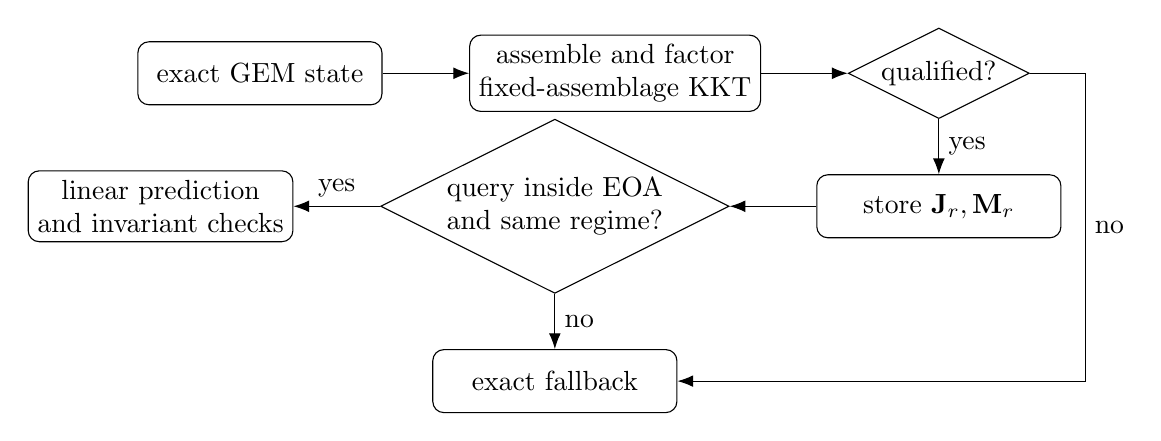
\begin{tikzpicture}[node distance=7mm and 11mm,
    box/.style={draw,rounded corners,align=center,minimum width=31mm,minimum height=8mm},
    decision/.style={draw,diamond,aspect=2,align=center,inner sep=1pt},
    flow/.style={-{Latex[length=2mm]}}]
    \node[box] (exact) {exact GEM state};
    \node[box,right=of exact] (kkt) {assemble and factor\\fixed-assemblage KKT};
    \node[decision,right=of kkt] (valid) {qualified?};
    \node[box,below=of valid] (record) {store $\mathbf{J}_r,\mathbf{M}_r$};
    \node[decision,left=of record] (inside) {query inside EOA\\and same regime?};
    \node[box,left=of inside] (predict) {linear prediction\\and invariant checks};
    \node[box,below=of inside] (fallback) {exact fallback};
    \draw[flow] (exact)--(kkt);
    \draw[flow] (kkt)--(valid);
    \draw[flow] (valid)--node[right]{yes}(record);
    \draw[flow] (record)--(inside);
    \draw[flow] (inside)--node[above]{yes}(predict);
    \draw[flow] (inside)--node[right]{no}(fallback);
    \draw[flow] (valid.east) -- ++(7mm,0) |- node[pos=0.25,right]{no} (fallback.east);
  \end{tikzpicture}
  \caption{Construction and use of a KKT-linear cache record.}
  \label{fig:kkt-flow}
\end{figure}

\section{Auditing and exact fallback}

Let $M$ be \code{surrogate\_audit\_interval}.  Accepted approximate predictions are numbered
locally within each worker.  When $M>0$, every $M$th accepted prediction is recomputed exactly:
\begin{equation}
  p\bmod M=0,
  \label{eq:audit-schedule}
\end{equation}
where $p$ is the worker's accepted-prediction count.  The exact value, never the approximate value,
is published for an audited state.  For each output the audit applies the physical-unit test
\begin{equation}
  \abs{\widehat y_j-y_j^{\mathrm{exact}}}
  \leq \varepsilon_{a,j}
  +\varepsilon_r\max\left(
    \abs{\widehat y_j},\abs{y_j^{\mathrm{exact}}}
  \right).
  \label{eq:audit-test}
\end{equation}
An audit failure increments telemetry but does not terminate the application.  The exact result is
cached if capacity remains.  Setting $M=0$ disables auditing.

Any empty-cache, insufficient-neighbor, phase, geometry, empirical-error, or invariant rejection
falls back to Equation~\eqref{eq:gem}.  A successful exact calculation is evaluated for all
requested outputs and inserted into the cache while capacity remains.  If the exact GEM fails, the
normal Thermochimica error path is used.

\section{Exact-solve warm starts}

Surrogate acceptance determines whether GEM is needed; warm-start selection determines how a GEM
call is initialized.  The available modes are:
\begin{description}[style=nextline]
  \item[\code{none}] Do not request Thermochimica reinitialization.
  \item[\code{previous\_solve}] Reuse the preceding solve in the same worker.
  \item[\code{previous\_timestep}] Reuse stored reinitialization data for the same mesh entity.
  \item[\code{nearest\_cached}] Load reinitialization data from the nearest normalized exact cache
  record.
\end{description}

For \code{nearest\_cached}, the currently implemented rescaling copies the cached reinitialization
record and multiplies its \code{molesPhase} entries by
\begin{equation}
  \rho=\frac{s_{\mathrm{query}}}{s_{\mathrm{record}}}.
  \label{eq:warm-rescale}
\end{equation}
If this warm GEM call fails, Thermochimica state and reinitialization data are reset and the same
state is retried once without reinitialization.  The retry is counted as an additional exact solve
and as a cold retry.  Warm starts affect computational cost, but a converged exact solve is expected
to represent the same equilibrium map $\mathcal{F}$.

\section{Control flow}

Figure~\ref{fig:flow} shows the decision path for one state.  ``Return prediction'' means that no
GEM call is made.  An audit deliberately follows the exact branch and publishes the exact output.

\begin{figure}[htbp]
  \centering
  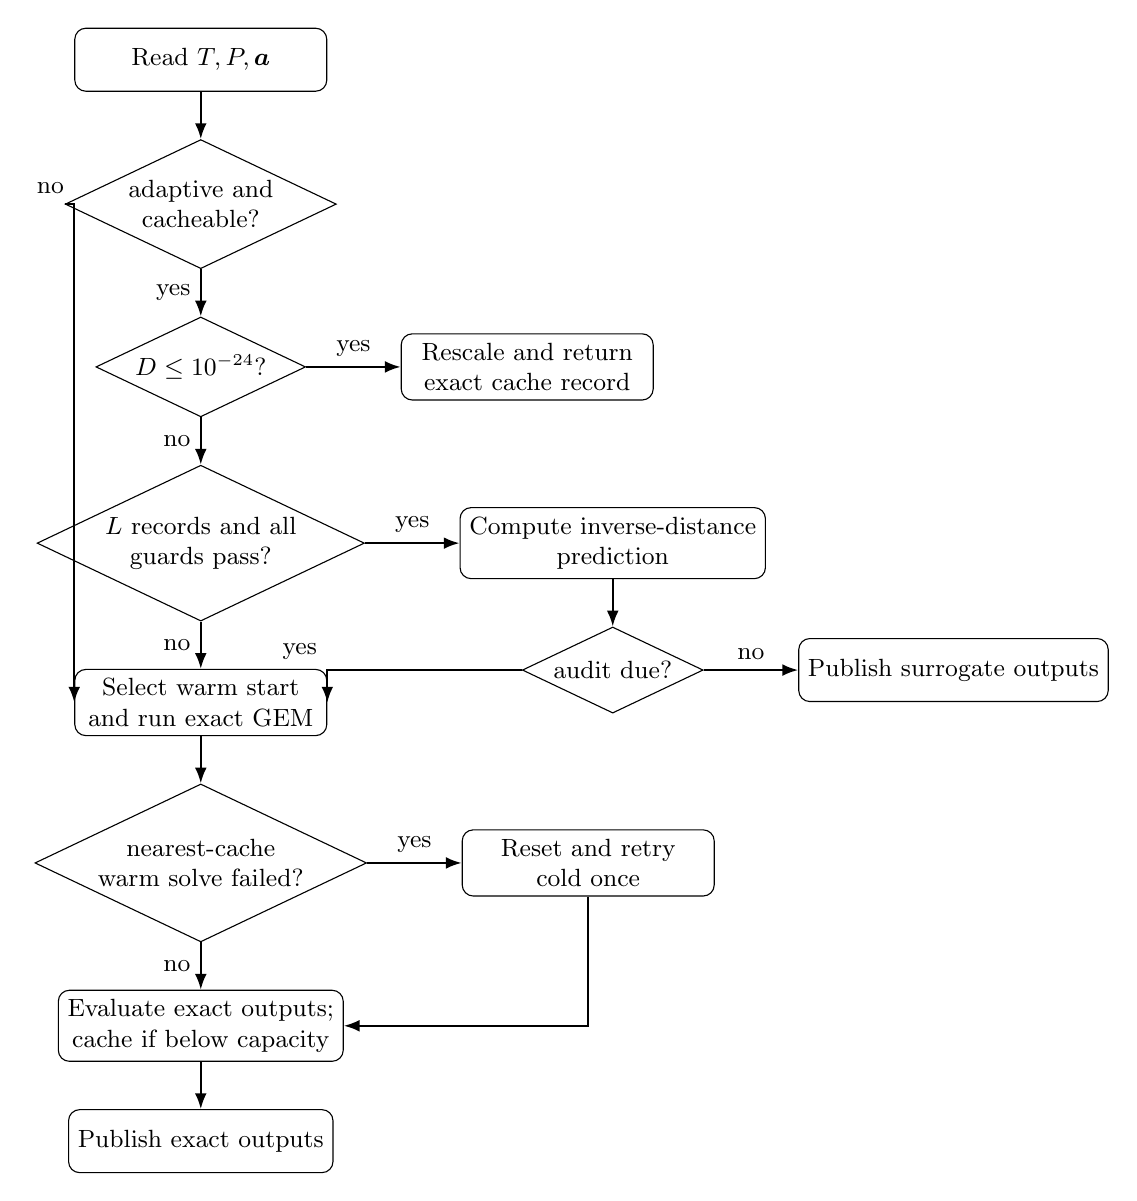
\begin{tikzpicture}[
    node distance=6mm and 12mm,
    font=\small,
    box/.style={draw, rounded corners, align=center, minimum width=32mm, minimum height=8mm},
    decision/.style={draw, diamond, aspect=2.1, align=center, inner sep=1.5pt},
    arrow/.style={-{Latex[length=2mm]}, thick}
  ]
    \node[box] (input) {Read $T,P,\boldsymbol{a}$};
    \node[decision, below=of input] (mode) {adaptive and\\cacheable?};
    \node[decision, below=of mode] (same) {$D\leq10^{-24}$?};
    \node[box, right=of same] (reuse) {Rescale and return\\exact cache record};
    \node[decision, below=of same] (guards) {$L$ records and all\\guards pass?};
    \node[box, right=of guards] (predict) {Compute inverse-distance\\prediction};
    \node[decision, below=of predict] (audit) {audit due?};
    \node[box, below=of guards] (gem) {Select warm start\\and run exact GEM};
    \node[decision, below=of gem] (retry) {nearest-cache\\warm solve failed?};
    \node[box, right=of retry] (cold) {Reset and retry\\cold once};
    \node[box, below=of retry] (store) {Evaluate exact outputs;\\cache if below capacity};
    \node[box, below=of store] (return) {Publish exact outputs};
    \node[box, right=of audit] (surrogate) {Publish surrogate outputs};

    \draw[arrow] (input) -- (mode);
    \draw[arrow] (mode) -- node[left]{yes} (same);
    \draw[arrow] (mode.west) -| node[above left]{no} (gem.west);
    \draw[arrow] (same) -- node[above]{yes} (reuse);
    \draw[arrow] (same) -- node[left]{no} (guards);
    \draw[arrow] (guards) -- node[above]{yes} (predict);
    \draw[arrow] (guards) -- node[left]{no} (gem);
    \draw[arrow] (predict) -- (audit);
    \draw[arrow] (audit) -- node[above]{no} (surrogate);
    \draw[arrow] (audit.west) -| node[above left]{yes} (gem.east);
    \draw[arrow] (gem) -- (retry);
    \draw[arrow] (retry) -- node[above]{yes} (cold);
    \draw[arrow] (retry) -- node[left]{no} (store);
    \draw[arrow] (cold) |- (store);
    \draw[arrow] (store) -- (return);
  \end{tikzpicture}
  \caption{Per-state adaptive execution flow.  Exact mode enters the GEM branch directly.}
  \label{fig:flow}
\end{figure}

The acceptance funnel in Figure~\ref{fig:funnel} emphasizes that each test is conjunctive.  A
prediction is usable only if it survives every layer.

\begin{figure}[htbp]
  \centering
  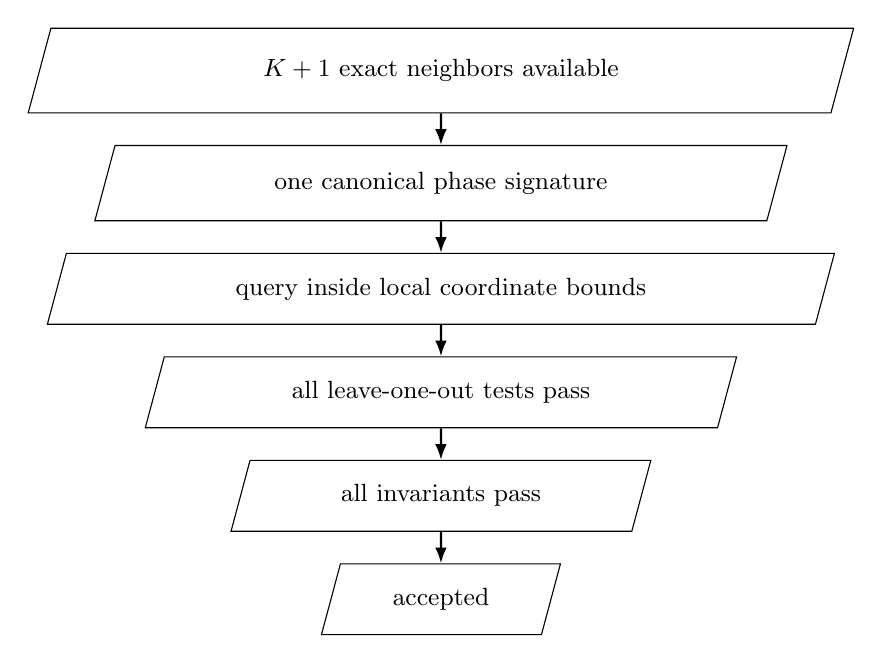
\begin{tikzpicture}[
    font=\small,
    stage/.style={draw, trapezium, trapezium left angle=75, trapezium right angle=105,
                  align=center, minimum height=9mm},
    node distance=4mm,
    arrow/.style={-{Latex[length=2mm]}, thick}
  ]
    \node[stage, minimum width=105mm] (enough) {$K+1$ exact neighbors available};
    \node[stage, minimum width=88mm, below=of enough] (phase) {one canonical phase signature};
    \node[stage, minimum width=72mm, below=of phase] (geometry) {query inside local coordinate bounds};
    \node[stage, minimum width=57mm, below=of geometry] (loo) {all leave-one-out tests pass};
    \node[stage, minimum width=43mm, below=of loo] (invariant) {all invariants pass};
    \node[stage, minimum width=29mm, below=of invariant] (accepted) {accepted};
    \draw[arrow] (enough) -- (phase);
    \draw[arrow] (phase) -- (geometry);
    \draw[arrow] (geometry) -- (loo);
    \draw[arrow] (loo) -- (invariant);
    \draw[arrow] (invariant) -- (accepted);
  \end{tikzpicture}
  \caption{Adaptive acceptance funnel.  Rejection at any level triggers an exact solve.}
  \label{fig:funnel}
\end{figure}

\subsection{Reference pseudocode}

Listing~\ref{lst:state-evaluation} expresses the implemented per-state decision order.  The order
is significant: exact identity is tested before approximate retrieval, audited predictions enter
the exact path, exact outputs are published even when an audit fails, and only successful exact
states can extend the table.

\begin{lstlisting}[caption={Safeguarded evaluation of one thermochemical state.},
label={lst:state-evaluation}]
function evaluate(state):
    key, scale, cacheable = normalize(state)
    if adaptive and cacheable:
        prediction = retrieve_exact_or_surrogate(key, scale)
        if prediction.accepted and not prediction.audit_due:
            return prediction.outputs

    set_T_P_and_element_amounts(state)
    select_warm_start()
    status = full_GEM()
    if status != 0 and nearest_cache_warm_start_was_used:
        reset_all_thermo_state()
        status = full_GEM_without_reinitialization()
    require(status == 0)

    exact = evaluate_all_requested_outputs()
    if prediction.audit_due:
        compare(prediction.outputs, exact)
        if KKT and audit_failed:
            shrink_source_ellipsoid()

    if KKT and an_existing_record_predicts_exact_within_tolerance:
        grow_that_ellipsoid()
    else if cache_has_capacity:
        cache_exact_state_and_optional_sensitivity()
    return exact
\end{lstlisting}

The local interpolation validator is summarized in
Listing~\ref{lst:idw-validation}.  The implementation rejects at the first failed category, so
the rejection counters form an ordered diagnostic rather than independent event counts.

\begin{lstlisting}[caption={Local inverse-distance validation and retrieval.},
label={lst:idw-validation}]
cloud = K_plus_one_nearest_exact_records(query)
require(size(cloud) == K + 1)
require(all phase_signatures_are_equal(cloud))
require(query_inside_coordinatewise_cloud_bounds(cloud))

for held_record in cloud:
    reconstructed = IDW(cloud excluding held_record)
    require(all_outputs_within_tolerance(held_record, reconstructed))

prediction = IDW(cloud)
require(all_outputs_finite_and_physically_admissible(prediction))
return prediction
\end{lstlisting}

Listing~\ref{lst:kkt-construction} shows the KKT record construction at the level needed to
reproduce its numerical safeguards.  The residual differences perturb the thermodynamic state
without additional GEM iterations; the converged state is restored after every construction or
trial evaluation.

\begin{lstlisting}[caption={Construction of a fixed-assemblage KKT cache record.},
label={lst:kkt-construction}]
require(all_system_solution_models_are_qualified())
snapshot = capture_converged_thermochimica_state()
R0 = fixed_assemblage_residual(snapshot)
require(scaled_norm(R0) <= 10 * solver_tolerance)

K = dR_d(log_active_amounts, element_potentials)
C = dR_d(T, P, elemental_amounts)
equilibrate_rows_and_columns(K, C)
require(reciprocal_condition_number(K) >= 1e-12)
dw_du = solve(K, -C)                  # all parameter right-hand sides
require(linear_residual_and_backward_error_are_acceptable())

J_output = centered_output_differences_using(dw_du)
M = identity + transpose(J_output) * W^2 * J_output
restore(snapshot)
store(J_output, M, state_amount_jacobian, regime_token)
\end{lstlisting}

\clearpage

\section{Telemetry and interpretation}

When \code{report\_performance=true}, MOOSE reports state and timing counters aggregated from its
worker processes.  The adaptive-specific quantities have the following meanings:
\begin{itemize}[leftmargin=*]
  \item \code{exact\_solves}: Thermochimica calls, including a cold retry after a failed nearest
  warm start;
  \item \code{gem\_iterations}: iterations reported in saved reinitialization data;
  \item \code{exact\_reuse\_hits}: identical normalized cache lookups;
  \item \code{surrogate\_hits}: accepted and published approximate results; audited predictions
  are not included;
  \item \code{phase}, \code{geometry}, \code{error}, \code{invariant}, and
  \code{invalid\_state} rejections: the first failed guard for a state;
  \item \code{audits} and \code{audit\_failures}: exact checks and failures of
  Equation~\eqref{eq:audit-test};
  \item \code{nearest\_warm\_starts} and \code{cold\_retries}: cache-based exact initializations
  and their fallback retries; and
  \item \code{cache\_entries} and \code{cache\_saturated}: current occupancy and whether admission
  capacity has been reached.
\end{itemize}
An exact-solve counter is a call count rather than a state count, because one state can incur a
warm attempt and a cold retry.  Worker solve time excludes parent-side packing and interprocess
communication, which are reported separately.  Since caches and audit sequences are worker-local,
thread or MPI decompositions can change hit counts without changing the configured algorithm.

\section{Computational cost}

\subsection{Notation and exact-solve baseline}

Let \(N\) be the number of query states, \(C\) the exact-record count in one worker, \(n\) the
number of chemical elements, \(d=n+2\) the cache-coordinate dimension, \(m\) the requested-output
count, \(K\) the requested neighbor count, \(L=K+1\), \(a\) the number of active phase/species
amounts in a KKT record, and \(v=a+n\) the approximate KKT system order.  Denote the average full
GEM cost by \(t_G\), the surrogate retrieval cost by \(t_S\), the fixed per-launch cost by
\(t_0\), and non-GEM per-state framework work by \(t_F\).

Exact query-stage time is modeled as
\begin{equation}
  T_{\mathrm{exact}}(N)\simeq t_0+N(t_F+t_G).
  \label{eq:exact-cost-model}
\end{equation}
The GEM term is not assigned a universal polynomial order because phase selection, solution-model
evaluation, subminimization, nonlinear iterations, and active-set changes depend strongly on the
database and thermodynamic state.  Measured GEM iterations and wall time are therefore more
informative than an asymptotic expression in \(n\) alone.

\subsection{Local inverse-distance interpolation}

Balanced \(k\)-d-tree lookup is typically \(O(\log C+K)\) in favorable low-dimensional data, but
the worst case is \(O(C)\), and the advantage can collapse as \(d\) increases.  After lookup, the
phase and bounding-box guards cost \(O(Ld)\).  Direct leave-one-out reconstruction computes
pairwise distances and all outputs, costing
\begin{equation}
  T_{\mathrm{LOO}}=O\!\left(L^2(d+m)\right).
\end{equation}
The final query interpolation is \(O(L(d+m))\).  With the automatic
\(K=\max(2d+1,8)\), the validation term is \(O(d^2(d+m))\), or \(O(d^3)\) when \(m\) is bounded or
proportional to \(d\).  This cubic coordinate-dimension dependence is inexpensive only while
GEM remains substantially more costly.

If fractions \(\phi_R,\phi_A,\phi_F\) of query states are exact reuses, audited predictions, and
fallbacks, respectively, the exact-call fraction is approximately
\begin{equation}
  f_G = \phi_A+\phi_F+\phi_{\mathrm{retry}},
  \qquad
  T_{\mathrm{adaptive}}\simeq t_0+N\left[t_F+
  (1-\phi_R-\phi_A-\phi_F)t_S+f_Gt_G\right].
  \label{eq:adaptive-cost-model}
\end{equation}
For an audit interval \(M\), a perfectly accepted trajectory with no exact reuse or fallback has
the upper bound \(1-f_G\approx1-1/M\) on exact-call reduction.  Thus the 0.898--0.900 reductions
observed with \(M=10\) are the expected audit-limited plateau, not unexplained residual work.

An IDW cache record stores coordinates, normalized outputs, phase metadata, and optionally a
reinitialization state.  Excluding allocator overhead and integer tokens, its floating-point
storage is \(O(d+m+r)\), where \(r\) is reinitialization size.  Total worker storage is
\(O(C(d+m+r))\).

\subsection{KKT sensitivity construction and retrieval}

One KKT construction evaluates residual perturbations for active solution constituents and for
temperature and pressure, forms an order-\(v\) dense system, estimates conditioning, solves \(d\)
right-hand sides, and builds requested-output derivatives.  A useful leading-order model is
\begin{equation}
  T_{\mathrm{build}} =
  O\!\left(a\,T_R+v^3+v^2d+d\,T_Y\right),
\end{equation}
where \(T_R\) is one fixed-assemblage residual evaluation and \(T_Y\) is one pass through all output
getters.  Unlike finite differences of GEM, these perturbations do not rerun the nonlinear
equilibrium solver.

For each candidate record, the ellipsoid test is \(O(d^2)\); evaluation of the state and output
linearizations is \(O((a+m)d)\).  Searching \(K\) candidate records is therefore
\begin{equation}
  T_{\mathrm{retrieve}} =
  O\!\left(T_{\mathrm{tree}}+Kd^2+(a+m)d\right).
\end{equation}
With automatic \(K=O(d)\), the metric tests can again become \(O(d^3)\).  A rank-one ellipsoid
growth or shrink costs \(O(d^2)\).

The dominant floating-point storage in one sensitivity record is
\begin{equation}
  B_{\mathrm{KKT}}\approx 8\left[d+m+md+d^2+a+ad\right]\ {\rm bytes},
  \label{eq:kkt-storage}
\end{equation}
before vector capacity, integer regime tokens, tree storage, and optional reinitialization data.
The \(d^2\) metric and the \(d(m+a)\) Jacobians make KKT cache memory materially more sensitive to
chemical dimension than IDW memory.  Because caches are worker-local, aggregate storage is
approximately proportional to the number of active MOOSE workers.

\subsection{Wall-time ceiling and parallel scaling}

If a fraction \(f\) of exact wall time is actually removable GEM work and that portion is
accelerated by \(S_G\), Amdahl's law gives
\begin{equation}
  S_{\mathrm{wall}}\leq
  \frac{1}{(1-f)+f/S_G}.
  \label{eq:amdahl}
\end{equation}
This explains why a sevenfold worker-time reduction can coexist with a wall speedup below two for
cheap Mo--Ru equilibria at only 1,000 states.  Process startup, mesh work, field packing, IPC,
sampling, and output remain.  Larger or chemically more expensive problems increase \(f\), while
surrogate validation, memory traffic, and cache saturation can reduce it.

For fixed total state count and \(p\) workers, ideal strong scaling would give
\(T_p\simeq T_1/p\) and efficiency \(E_p=T_1/(pT_p)\).  In the present design each worker receives
only its local state trajectory and must independently obtain enough exact records.  Increasing
\(p\) can therefore:
\begin{itemize}[leftmargin=*]
  \item reduce local point density below the \(K\) or ellipsoid requirement;
  \item replicate cache population and KKT factorization;
  \item change deterministic audit positions;
  \item multiply memory by approximately \(p\); and
  \item add MPI and worker-process communication.
\end{itemize}
Parallel efficiency must consequently be reported together with exact calls per state, utilization
fractions, cache entries, and peak resident memory.  Timing alone cannot distinguish useful
parallel GEM work from loss of surrogate coverage.

\section{Algorithm-comparison metrics}

The benchmark suite compares exact GEM, \code{local\_idw}, and \code{kkt\_linear} on a balanced
set of problems.  For output $j$ on problem $p$, it reports the normalized error
\begin{equation}
  \eta_{p,j} =
  \frac{
    \max_i \lvert \widehat y_{p,i,j} - y_{p,i,j} \rvert
  }{
    \epsilon_{\mathrm{abs},j}
    + \epsilon_{\mathrm{rel}}
      \max_i\left(\lvert y_{p,i,j}\rvert,
                  \lvert \widehat y_{p,i,j}\rvert\right)
  },
  \qquad
  \eta_p = \max_j \eta_{p,j}.
  \label{eq:benchmark-normalized-error}
\end{equation}
A result is considered valid when $\eta_p\leq 1$, no audit fails, and no state-restoration
failure is reported.  Invalid results remain visible in work--precision diagrams but receive
infinite cost in the profiles below.

For valid algorithm $a$, let $t_{p,a}$ be its median query-stage time and define its performance
ratio relative to the fastest valid algorithm on the same problem,
\begin{equation}
  r_{p,a} = \frac{t_{p,a}}{\min_{a'\in\mathcal V_p}t_{p,a'}}.
\end{equation}
The Dolan--Mor\'e performance profile is
\begin{equation}
  \rho_a(\tau) =
  \frac{1}{\lvert\mathcal P\rvert}
  \left\lvert
    \left\{p\in\mathcal P:r_{p,a}\leq\tau\right\}
  \right\rvert .
  \label{eq:performance-profile}
\end{equation}
Thus $\rho_a(1)$ is the fraction of problems on which $a$ is fastest, while the large-$\tau$
limit is the fraction solved within tolerance.  Separate worker-time and wall-time profiles
distinguish equilibrium cost from application overhead.

The data profile replaces time with the normalized exact-solve budget
\begin{equation}
  \beta_{p,a} =
  \frac{N^{\mathrm{GEM}}_{p,a}}{N^{\mathrm{state}}_p},
  \qquad
  d_a(\beta) =
  \frac{1}{\lvert\mathcal P\rvert}
  \left\lvert
    \left\{p\in\mathcal P:\beta_{p,a}\leq\beta\right\}
  \right\rvert .
  \label{eq:data-profile}
\end{equation}
This shows how rapidly each method covers the problem set as the permitted GEM calls per state
increase.  Work--precision plots retain the individual $(\eta_p,t_{p,a})$ points, heat maps
summarize speedup by chemistry and model, stage-learning plots show cache growth and exact-call
fraction, and phase-trajectory plots place surrogate error directly against the exact phase
fractions.  Together these views avoid declaring a method superior from timing alone when it
does not satisfy the requested thermodynamic accuracy.

\section{Experimental methodology and evidence}

\subsection{Evidence classes}

This report deliberately separates four classes of evidence:
\begin{longtable}{L{0.18\textwidth}L{0.31\textwidth}L{0.43\textwidth}}
  \caption{Evidence classes and permitted interpretation.}
  \label{tab:evidence-classes}\\
  \toprule
  Class & Source & Interpretation \\
  \midrule
  \endfirsthead
  \toprule
  Class & Source & Interpretation \\
  \midrule
  \endhead
  Implementation fact &
  C++, Fortran, Python, manifests, and inputs at parent revision
  \code{93d6ca63a5} and Thermochimica revision \code{b1519a75b6} &
  Supports algorithm, control-flow, and complexity statements; does not establish speed. \\
  Repository qualification observation &
  Exact scans and local timings documented in \code{BENCHMARK\_INVENTORY.md} &
  Supports case design and launch planning; hardware-specific and not a production result. \\
  Previous HPC campaign &
  \code{failures (2).csv}, 144 rows &
  Supports diagnosis of a pre-solve launch defect only; contains no valid performance sample. \\
  Local exploratory measurement &
  One repetition per configuration on macOS arm64, 12 logical CPUs, 28 July 2026 &
  Supports repaired-path behavior and order-of-magnitude discussion; does not support confidence
  intervals or portable HPC claims. \\
  \bottomrule
\end{longtable}

The local exploratory runs used the existing \code{chemical\_reactions-opt} executable, the quick
manifest, no priming launch, and one measured repetition.  The benchmark smoke validation and all
nine Python driver unit tests passed.  The local result metadata recorded a clean parent worktree,
Python 3.14.6, and the source revision above.  Because the metadata records the executable only by
path, these observations should be regarded as a validation of the checked-out workflow rather
than a cryptographically reproducible binary experiment.

\subsection{Case matrix}

The study design correctly distinguishes smooth performance, phase-boundary safety, model
qualification coverage, and scaling:
\begin{itemize}[leftmargin=*]
  \item fixed-HCP Mo--Ru isolates best-case interpolation and KKT retrieval in a qualified
  \code{QKTO} model;
  \item restricted HCP, HCP+liquid, liquid, BCC+liquid, and BCC intervals plus a full traversal
  create a common-output capability matrix;
  \item LiF-carrier trace additions vary chemical dimension through 2, 5, 9, 13, and 17 elements;
  \item excess-F Li--F, low-temperature LiF, and active-MSFL FLiBe are state-isolation and
  unsupported-model regressions, not performance cases;
  \item representative MSRE-derived fluoride evaluates high-dimensional GEM cost and IDW coverage;
  and
  \item a heat-capacity variant isolates derived outputs that invoke additional equilibria.
\end{itemize}
The full manifest requests seven measured repetitions after one unmeasured prime.  Medians and
interquartile ranges are appropriate for the mildly skewed timing distributions expected on an HPC
system; publication runs should additionally report node allocation, affinity, frequency policy,
compiler, MPI, and aggregate process-tree memory.

\subsection{Accuracy and capability gates}

Exact warm-start and exact cold-start samples are compared before either adaptive method runs.
The output-specific absolute floor is the larger of ten times their reproducibility difference
and a floating-point precision floor.  This avoids using adaptive results to choose their own
tolerance and makes near-zero phase amounts meaningful in Equation~\eqref{eq:benchmark-normalized-error}.

The implemented capability gate is conjunctive:
\begin{equation}
  \eta_p\leq1,\quad N_{\mathrm{audit\ fail}}=0,\quad
  N_{\mathrm{restore\ fail}}=0,\quad
  1-\frac{N_{\mathrm{GEM,adaptive}}}{N_{\mathrm{GEM,exact}}}\geq0.5,\quad
  \frac{T_{\mathrm{wall,exact}}}{T_{\mathrm{wall,adaptive}}}\geq2.
  \label{eq:capability-gate}
\end{equation}
The Python implementation uses total wall speedup in the final condition.  Some inventory text
still describes a twofold \emph{worker}-time criterion and should be reconciled before publication.
Worker speedup remains a valuable diagnostic, but it cannot pass the current software gate.

\section{Results and discussion}

\subsection{Disposition of the previous HPC campaign}

The available failure file contains exactly 144 rows: six Mo--Ru phase-regime problems, three mesh
sizes, four relative tolerances, and two surrogate models.  Every configuration failed before an
equilibrium solve because the cold exact-calibration command supplied
\code{surrogate\_model=calibration}; the MOOSE enum accepts only \code{local\_idw} and
\code{kkt\_linear}.  The failure distribution is therefore \(144/144\) with one common root cause.
No failed row may be included in timing averages, performance profiles, or accuracy statistics.

Commit \code{35dd47245d} repairs this path by assigning the valid \code{local\_idw} enum to the cold
configuration while retaining \code{acceleration=exact}.  Exact execution does not use the
surrogate, but input parsing still validates its enum.  The repaired smoke suite completed
successfully, and the local exploratory capability campaign completed all configurations with an
empty failure table.  The correct scientific treatment is to archive the failed campaign as an
excluded preflight attempt and rerun the full array; it is not a negative performance result.

\subsection{Exploratory common-capability results}

Table~\ref{tab:local-capability} reports the one-repetition, 1,000-state, \(10^{-4}\)-tolerance
comparison.  \(S_w\) is total wall speedup, \(S_G\) is worker solve-time speedup, \(R_G\) is exact
GEM call reduction, \(\eta_{\max}\) is the worst normalized sampled-output error, and \(F\) is the
exact-fallback fraction of query states.  Audit states are not included in \(F\).  All twelve
adaptive configurations had zero audit failures and zero state-restoration failures.

\begin{table}[htbp]
  \centering
  \caption{Local exploratory capability results at \(N=1000\) and
  \(\varepsilon_r=10^{-4}\).  One repetition; values are not production statistics.}
  \label{tab:local-capability}
  \small
  \begin{tabular}{llrrrrr}
    \toprule
    Regime & Method & \(S_w\) & \(S_G\) & \(R_G\) & \(\eta_{\max}\) & \(F\) \\
    \midrule
    HCP & IDW & 1.12 & 2.03 & 0.534 & 0.000 & 0.407 \\
    HCP & KKT & 1.40 & 7.35 & 0.898 & 0.762 & 0.002 \\
    HCP+liquid & IDW & 0.97 & 0.91 & 0.000 & 0.000 & 1.000 \\
    HCP+liquid & KKT & 0.83 & 0.62 & 0.537 & 0.581 & 0.403 \\
    liquid & IDW & 1.31 & 6.72 & 0.898 & 0.025 & 0.002 \\
    liquid & KKT & 1.43 & 7.51 & 0.900 & 0.726 & 0.000 \\
    BCC+liquid & IDW & 0.97 & 0.92 & 0.000 & 0.000 & 1.000 \\
    BCC+liquid & KKT & 0.81 & 0.58 & 0.469 & 0.633 & 0.478 \\
    BCC & IDW & 1.41 & 7.07 & 0.898 & 0.035 & 0.002 \\
    BCC & KKT & 1.62 & 7.54 & 0.898 & 0.786 & 0.002 \\
    full traversal & IDW & 0.99 & 1.03 & 0.055 & 0.000 & 0.939 \\
    full traversal & KKT & 1.12 & 2.59 & 0.726 & 0.767 & 0.193 \\
    \bottomrule
  \end{tabular}
\end{table}

Three conclusions follow.  First, KKT retrieval reaches the audit-limited exact-call reduction in
the smooth single-phase HCP, liquid, and BCC intervals and reduces worker time by about
\(7.3\)--\(7.5\).  Its normalized errors of 0.73--0.79 are below, but intentionally closer to, the
acceptance boundary than the highly conservative IDW errors.  Second, neither algorithm obtains a
twofold total wall speedup at 1,000 states.  Full GEM wall times are only 0.50--0.77~s and worker
solve times only 0.045--0.136~s, leaving most of the launch in non-GEM work.  Third, mixed-phase
windows expose different conservatism: IDW falls back for every query in both two-phase intervals,
whereas KKT accepts a useful fraction but its sensitivity-construction and rejection overhead
outweigh the cheap avoided GEMs at this scale.

For the full traversal, local IDW rejects predominantly through its local empirical-error test and
performs essentially like exact GEM.  KKT reduces exact calls by 72.6\% and worker time by a factor
of 2.59 while retaining exact fallback for 19.3\% and auditing 8.1\% of query states.  This is the
desired qualitative boundary behavior: acceptance within a stable regime, fallback near active-set
changes, and exact published values for audits.

\subsection{State-count scaling and grid aliasing}

Table~\ref{tab:mesh-scaling} summarizes the quick fixed-HCP mesh study.  Exact worker time is close
to linear: a least-squares descriptive model is
\begin{equation}
  T_{\mathrm{worker,exact}}\simeq
  9.94\times10^{-3}+9.92\times10^{-5}N\ {\rm s},
  \qquad R^2=0.9999.
\end{equation}
Total wall time is similarly described by
\begin{equation}
  T_{\mathrm{wall,exact}}\simeq
  0.346+3.26\times10^{-4}N\ {\rm s},
  \qquad R^2=0.9999.
\end{equation}
These fits are descriptive for one local run, but they quantify the large fixed and non-GEM
per-state costs responsible for the wall-time ceiling.

\begin{table}[htbp]
  \centering
  \caption{Local exploratory fixed-HCP state-count study.  One repetition.}
  \label{tab:mesh-scaling}
  \small
  \begin{tabular}{rrrrrrrr}
    \toprule
    \(N\) & \(T_w^{\rm exact}\) & \(T_w^{\rm adap}\) &
    \(T_G^{\rm exact}\) & \(T_G^{\rm adap}\) &
    GEM calls & surrogate & exact reuse \\
    & (s) & (s) & (s) & (s) & & hits & hits \\
    \midrule
    100 & 0.364 & 0.363 & 0.0138 & 0.0140 & 100 & 0 & 0 \\
    1,000 & 0.688 & 0.592 & 0.1158 & 0.00613 & 17 & 983 & 0 \\
    10,000 & 3.602 & 1.647 & 1.0015 & 0.01466 & 74 & 0 & 9,926 \\
    \bottomrule
  \end{tabular}
\end{table}

The 10,000-state point is not a clean interpolation-scaling result.  For the final query stage,
\code{binary\_smooth.i} changes Mo amount by
\(\Delta a_{\rm Mo}=2(0.00037)=0.00074\) over a trajectory span of 0.1.  The displacement in mesh
cells is therefore
\begin{equation}
  q_N=\frac{\Delta a_{\rm Mo}}{0.1}N=0.0074N.
\end{equation}
At \(N=10{,}000\), \(q_N=74\) is integral, so all but the 74 newly exposed edge states coincide
with populated cache coordinates.  The full-manifest points 30,000 and 100,000 similarly give 222
and 740 cells.  Their apparent exact-call reductions and lookup speedups measure exact reuse, not
IDW accuracy or cost.  The capability-comparison generator already avoids this defect by using an
irrational, non-grid-aligned displacement and explicitly rejecting overlap.  The mesh study should
reuse that mechanism before its upper points are interpreted as surrogate scaling.

At \(N=100\), the local cloud is too coarse to satisfy the \(10^{-4}\) leave-one-out criterion:
99 queries are error rejections and one is a geometry rejection.  At \(N=1{,}000\), local density
is sufficient; only 17 exact calls remain, including nine scheduled audits, and no audit fails.
This illustrates a genuine crossover: increasing state density can make an in-situ local model
more useful even while the physical trajectory is unchanged.

\subsection{Neighborhood, auditing, and warm starts}

At 2,000 fixed-HCP states, explicit \(K=2\), \(K=8\), and automatic \(K=9\) produced the same 28
exact calls and 1,972 published surrogate hits.  Worker speedups decreased from 25.7 to 20.9 and
20.0 as local validation grew, whereas one-repetition wall speedups remained 1.63--1.67.  The
scientific expectation is that larger \(K\) can improve robustness when the cloud samples
curvature but increases \(O(L^2(d+m))\) validation work; there is no basis in these data for
choosing more than the smallest validated neighborhood on this one-dimensional trajectory.

Exact warm-start measurements at the same state count are summarized in
Table~\ref{tab:warm-start}.
\begin{table}[H]
  \centering
  \caption{Local exploratory exact-GEM warm-start comparison at \(N=2000\).}
  \label{tab:warm-start}
  \begin{tabular}{lrrr}
    \toprule
    Initialization & wall time (s) & worker time (s) & GEM iterations \\
    \midrule
    none & 1.598 & 0.406 & 54,486 \\
    previous solve & 1.044 & 0.220 & 26,011 \\
    previous timestep & 1.285 & 0.251 & 32,000 \\
    nearest cached & 1.046 & 0.208 & 22,022 \\
    \bottomrule
  \end{tabular}
\end{table}
Relative to no reinitialization, previous-solve, previous-timestep, and nearest-cache modes reduce
reported iterations by 52.3\%, 41.3\%, and 59.6\%, respectively.  Nearest-cache initialization has
the lowest worker time and iteration count in this trajectory, but it also retains reinitialization
records and incurs tree lookup.  Its failed warm attempts can cause one state to count two exact
solves; production results must report cold retries rather than infer state count from GEM calls.

With 2,000 states on the wide phase traversal, IDW reduced exact calls by 32.35\%, worker time by
1.59, and wall time by only 1.08.  It recorded 1,319 empirical-error rejections, 15 phase
rejections, 13 geometry rejections, six audits, and zero audit failures.  The predominance of
error rejection, rather than phase-token rejection, shows that equal phase signatures do not by
themselves make a cloud sufficiently smooth near a transition.  This is appropriate conservative
behavior, not a failed optimization.

\subsection{Chemical-dimension observations}

The repository records one-element-mesh exact initial/query times of approximately 0.4, 2.2, 6.3,
95--101, and 281~s for 2, 5, 9, 13, and 17 elements in MSTDB v4.1.  A 22-element run was stopped
after 952~s while still compute-bound.  A purely descriptive exponential fit to the five completed
points,
\begin{equation}
  T(n)\approx0.183\exp(0.444n)\ {\rm s},
  \qquad R^2\approx0.98,
\end{equation}
must not be interpreted as an algorithmic complexity law: adding trace elements also changes
candidate phases, active species, model evaluations, and nonlinear iteration paths.  It does,
however, justify the small 5--10-state fluoride grids and demonstrates why acceleration has much
greater potential wall-time leverage in representative chemistry than in cheap binary Mo--Ru.

The KKT implementation deliberately rejects the fluoride database because its set of solution
models includes unqualified \code{SUBQ}, \code{SUBL}, and related forms.  Expected successful
behavior is therefore positive \code{unsupported\_model\_rejections}, zero
\code{state\_restore\_failures}, exact output agreement, and no claimed KKT speedup.  IDW remains
eligible because it treats Thermochimica as a black-box exact map and validates only visited
outputs and phase signatures.

\subsection{Expected production results}

Subject to a corrected non-overlapping mesh trajectory and a successful seven-repetition HPC
campaign, the following outcomes are plausible and falsifiable:
\begin{enumerate}[leftmargin=*]
  \item Smooth qualified Mo--Ru regimes should show exact-call reductions approaching the
  audit-limited ceiling: about 90\% for \(M=10\) in the common capability study and about 99\% for
  \(M=100\) in fixed-HCP diagnostics.  KKT normalized errors should generally lie closer to unity
  than IDW errors because its ellipsoid is constructed from the requested tolerance.
  \item Wall speedup should increase with \(N\) only when avoided GEM work grows faster than
  framework, lookup, validation, memory, and output costs.  A worker speedup larger than two does
  not imply that the implemented wall-time gate will pass.
  \item Two-phase intervals and full phase traversals should have lower surrogate utilization and
  higher phase, geometry, complementarity, or empirical-error rejection.  Accuracy and zero audit
  failures take precedence over hit rate.
  \item Reducing tolerance should shrink accepted IDW clouds and KKT ellipsoids, increasing exact
  calls and time while decreasing absolute error.  A non-monotone tolerance curve is a diagnostic
  for sampling noise, cache-history changes, or phase-regime effects.
  \item Cache capacity below the number of useful regimes should cause saturation and a performance
  plateau because the first release has no eviction.  Capacity above the working set should add
  memory with little benefit.
  \item Audit overhead should be approximately proportional to \(1/M\) when acceptance is high.
  Audit failures, if any, should shrink KKT ellipsoids and must disqualify that configuration.
  \item Strong scaling should become subideal as worker-local caches fragment the trajectory and
  replicate training.  Exact calls per state and aggregate memory should generally rise with
  worker count unless the local state ordering remains especially favorable.
  \item Representative fluoride exact time should grow steeply with element set and requested
  derived outputs.  KKT should fail closed, while IDW speedup will depend on whether its
  \(O(d^3)\) local validation remains small compared with each avoided fluoride GEM.
\end{enumerate}

\section{Repository and benchmark quality assessment}

\subsection{Strengths}

\begin{itemize}[leftmargin=*]
  \item Exact mode is the default, and every adaptive rejection has a direct exact path.
  \item Worker-process isolation is a sound response to stateful Fortran modules and avoids
  thread-level corruption.
  \item Extensive outputs are normalized consistently with composition magnitude, preventing a
  cache trained at one total amount from silently mis-scaling integral properties.
  \item KKT construction checks base residual, conditioning, linear residual, backward error,
  active amounts, supported model type, active species, phase instances, miscibility, and state
  restoration.
  \item The benchmark compares complete output vectors against exact samples, includes near-zero
  absolute floors calibrated without adaptive data, and retains failed algorithms in profile
  denominators.
  \item Atomic CSV checkpoints, raw samples, logs, failure capture, and plot regeneration make long
  campaigns inspectable while running.
\end{itemize}

\subsection{Limitations and recommended corrections}

\begin{enumerate}[leftmargin=*]
  \item Replace the fixed-HCP mesh displacement with the same irrational, explicitly validated
  non-overlap construction used by \code{capability\_comparison}; invalidate the aliased 10,000,
  30,000, and 100,000 interpolation-scaling points from the present manifest.
  \item Record the executable SHA-256 digest, modification time, build method, compiler and linked
  library versions, parent revision, all submodule revisions, and an archived copy or digest of
  the selected manifest in \code{metadata.json}.
  \item Reconcile documentation that states a twofold worker-speed gate with the implemented
  twofold total-wall gate in Equation~\eqref{eq:capability-gate}.
  \item Repair or retire the upstream \code{TestSensitivity01} dependency on
  \path{examples/MSRE/MSTDB-TC_V3.0_Fluorides_No_Functions_8-2.dat}.  The file is absent in the
  current submodule checkout, and the prebuilt daily test reports failure.  The newer MOOSE v4.1
  safety regressions do not make an unexecutable upstream qualification test acceptable.
  \item Add an explicit build-source consistency preflight.  A clean Git worktree does not prove
  that an existing executable was built from that revision.
  \item Preserve the successful full result directory outside scheduler scratch and include raw
  samples, failures, metadata, manifests, Slurm logs, and figure-generation software versions.
\end{enumerate}

\section{Guarantees and limitations}

The safeguards provide empirical error control, not a mathematical error bound for every unaudited
query.  In particular:
\begin{itemize}[leftmargin=*]
  \item Leave-one-out consistency measures the observed local cloud; it cannot detect behavior not
  represented by those exact records.
  \item Equal neighbor signatures reduce phase-boundary risk, but they do not prove that the query
  has that assemblage.  The axis-aligned bounding box is also not a convex-hull test.
  \item The \code{local\_idw} coordinates use fixed reference scales and retain the redundant
  sum-to-one composition coordinate.  The \code{kkt\_linear} model removes that direction and
  learns an anisotropic metric, but only for a fixed phase assemblage.
  \item Positive interpolation weights preserve each neighbor output range but do not enforce
  coupled thermodynamic identities or elemental conservation between different output fields.
  \item Auditing is deterministic within a worker, but worker-local cache histories mean parallel
  runs need not audit or accept the same state sequence.
  \item A saturated cache stops learning.  It remains usable for lookup, but no eviction or
  replacement policy adapts it to later portions of the trajectory.
\end{itemize}

For validation or safety-critical calculations, use \code{acceleration=exact}.  The intended
capability gate for representative adaptive workloads is at least 50\% fewer GEM calls, at least a
factor-of-two reduction in total application wall time, and zero audit failures at relative
tolerance $10^{-4}$.  Meeting this empirical gate does not turn Equation~\eqref{eq:loo-test} into a
formal guarantee.

\section{Relation to adaptive tabulation literature}

The design follows the central in-situ adaptive-tabulation idea of Pope: retain information from
previous expensive evaluations, retrieve locally when an accuracy criterion is satisfied, and
otherwise evaluate exactly and grow the table~\cite{pope1997}.  Its equilibrium-specific motivation
is consistent with on-demand acceleration of chemical equilibrium calculations described by Leal
et al.~\cite{leal2020}.  Thermochimica's partitioning-of-Gibbs-energy formulation and intended
multiphysics coupling are described by Piro et al.~\cite{piro2013}.  The implementation offers both
a deliberately simple inverse-distance
predictor with an empirical leave-one-out test and the fixed-assemblage mapping gradient in
Equation~\eqref{eq:kkt-predictor}.  Its ellipsoid follows Pope's region-of-accuracy construction,
while exact audits and phase signatures provide the equilibrium-specific active-set safeguards.
For KKT retrieval, the implementation augments the phase signature with the indices of solution
constituents above Thermochimica's active mole-fraction threshold.  The two nearest records must
agree on this combined signature before any ellipsoid is considered.

The use of performance profiles follows Dolan and Mor\'e~\cite{dolan2002}.  In this application,
invalid or failed methods remain in the problem-set denominator and receive infinite cost.  This
detail is essential: otherwise, an aggressive method could appear faster merely by omitting the
phase regimes or tolerances it cannot solve accurately.

\begin{thebibliography}{9}
  \bibitem{pope1997}
  S. B. Pope,
  ``Computationally efficient implementation of combustion chemistry using in situ adaptive
  tabulation,''
  \emph{Combustion Theory and Modelling}, 1(1), 41--63, 1997.
  \url{https://doi.org/10.1080/713665229}

  \bibitem{leal2020}
  A. M. M. Leal, S. Kyas, D. A. Kulik, and M. O. Saar,
  ``Accelerating Reactive Transport Modeling: On-Demand Machine Learning Algorithm for Chemical
  Equilibrium Calculations,''
  \emph{Transport in Porous Media}, 133(2), 161--204, 2020.
  \url{https://doi.org/10.1007/s11242-020-01412-1}

  \bibitem{piro2013}
  M. H. A. Piro, S. Simunovic, T. M. Besmann, B. J. Lewis, and W. T. Thompson,
  ``The thermochemistry library Thermochimica,''
  \emph{Computational Materials Science}, 67, 266--272, 2013.
  \url{https://doi.org/10.1016/j.commatsci.2012.09.011}

  \bibitem{dolan2002}
  E. D. Dolan and J. J. Mor\'e,
  ``Benchmarking optimization software with performance profiles,''
  \emph{Mathematical Programming}, 91, 201--213, 2002.
  \url{https://doi.org/10.1007/s101070100263}
\end{thebibliography}

\appendix
\section{Configuration summary}

\begin{table}[htbp]
  \centering
  \caption{Adaptive controls and defaults.}
  \begin{tabular}{lll}
    \toprule
    Parameter & Default & Meaning \\
    \midrule
    \code{acceleration} & \code{exact} & exact or adaptive evaluation \\
    \code{surrogate\_model} & \code{local\_idw} & inverse-distance or KKT-linear mapping \\
    \code{cache\_max\_entries} & 10000 & exact records per worker \\
    \code{surrogate\_neighbors} & 0 & $K$, with zero selecting Equation~\eqref{eq:auto-k} \\
    \code{surrogate\_relative\_tolerance} & $10^{-4}$ & $\varepsilon_r$ \\
    \code{surrogate\_absolute\_tolerances} & zero by output & $\varepsilon_{a,j}$ \\
    \code{surrogate\_audit\_interval} & 100 & $M$, with zero disabling audits \\
    \bottomrule
  \end{tabular}
\end{table}

\section{Reproducibility listings}

The corrected smoke validation is:
\begin{lstlisting}[language=bash,caption={Functional validation of the benchmark workflow.}]
python3 modules/chemical_reactions/benchmarks/thermochimica_adaptive/benchmark.py \
  validate \
  --exe modules/chemical_reactions/chemical_reactions-opt
\end{lstlisting}

The production capability study and postprocessing sequence is:
\begin{lstlisting}[language=bash,caption={Full capability campaign and report generation.}]
python3 modules/chemical_reactions/benchmarks/thermochimica_adaptive/benchmark.py \
  run --tier full --study capability_comparison \
  --exe modules/chemical_reactions/chemical_reactions-opt \
  --output /persistent/path/capability-results

python3 modules/chemical_reactions/benchmarks/thermochimica_adaptive/benchmark.py \
  report --input /persistent/path/capability-results

python3 modules/chemical_reactions/benchmarks/thermochimica_adaptive/benchmark.py \
  plot --input /persistent/path/capability-results
\end{lstlisting}

The minimum archive required to reproduce a reported point is:
\begin{lstlisting}[caption={Required result artifacts.}]
runs.csv                 per-repetition, per-stage telemetry
accuracy.csv             exact-versus-adaptive output errors
summary.csv              median and interquartile range
comparison.csv           correctness-gated common capability table
capability_gate.csv      explicit pass/fail reason
utilization.csv          exact reuse / surrogate / audit / fallback partition
qualification.csv        unsupported-model and state-restoration results
failures.csv             all failed configurations
metadata.json            revision, platform, command, and environment
raw/                     sampled state outputs
logs/                    complete application logs
figures/                 publication graphics
\end{lstlisting}

\end{document}
